\documentclass[aspectratio=169]{beamer}
\usetheme[faculty=phil]{fibeamer}
\usepackage{polyglossia}
\setmainlanguage{english} %% main locale instead of `english`, you
%% can typeset the presentation in either Czech or Slovak,
%% respectively.
\setotherlanguages{russian} %% The additional keys allow
%%
%%   \begin{otherlanguage}{czech}   ... \end{otherlanguage}
%%   \begin{otherlanguage}{slovak}  ... \end{otherlanguage}
%%
%% These macros specify information about the presentation
\title[AGLA2]{Analytical Geometry and Linear Algebra II, Lab 7} %% that will be typeset on the
\subtitle{Complex numbers \\ Hermitian matrix \\ \ 
         } %% title page.
\author{Oleg Bulichev}
%% These additional packages are used within the document:
\usepackage{ragged2e}  % `\justifying` text
\usepackage{booktabs}  % Tables
\usepackage{tabularx}
\usepackage{tikz}      % Diagrams
\usetikzlibrary{calc, shapes, backgrounds}
\usepackage{amsmath, amssymb}
\usepackage{url}       % `\url`s
\usepackage{listings}  % Code listings
% \usepackage{subfigure}
\usepackage{floatrow}
\usepackage{subcaption}
\usepackage{mathtools}
\usepackage{todonotes}
\usepackage{fontspec}
\usepackage{multicol}
\usepackage{pdfpages}
\usepackage{wrapfig}
\usepackage{animate}

\graphicspath{{resources/}}
\frenchspacing

\setbeamertemplate{caption}[numbered]
\usetikzlibrary{graphs}

% \usepackage[backend=biber,style=ieee,autocite=footnote]{biblatex}
% \addbibresource{biblio.bib}
% \DefineBibliographyStrings{english}{%
%   bibliography = {References},}

\newcommand{\oleg}[2][] {\todo[color=red, #1] {OLEG:\\ #2}}
\newcommand{\fbckg}[1]{\usebackgroundtemplate{\includegraphics[width=\paperwidth]{#1}}}%frame background

\usepackage[framemethod=TikZ]{mdframed}
\newcommand{\dbox}[1]{
\begin{mdframed}[roundcorner=3pt, backgroundcolor=yellow, linewidth=0]
\vspace{1mm}
{#1}
\vspace{1mm}
\end{mdframed}
}

\begin{document}
\setlength{\abovedisplayskip}{0pt}
\setlength{\belowdisplayskip}{0pt}
\setlength{\abovedisplayshortskip}{0pt}
\setlength{\belowdisplayshortskip}{0pt}

\fbckg{fibeamer/figs/title_page.png}
\frame[c]{\setcounter{framenumber}{0}
    \usebeamerfont{title}%
    \usebeamercolor[fg]{title}%
    \begin{minipage}[b][6.5\baselineskip][b]{\textwidth}%
        \textcolor{black}{\raggedright\inserttitle}
    \end{minipage}
    % \vskip-1.5\baselineskip

    \usebeamerfont{subtitle}%
    \usebeamercolor[fg]{framesubtitle}%
    \begin{minipage}[b][3\baselineskip][b]{\textwidth}
        \raggedright%
        \insertsubtitle%
    \end{minipage}
    \vskip.25\baselineskip
}
%   \frame[c]{\maketitle}

\fbckg{fibeamer/figs/common.png}

\begin{frame}[t]{Complex numbers}
\framesubtitle{Representation}
\vspace{-0.5cm}
    \begin{columns}[T,onlytextwidth]
        \begin{column}{0.49\textwidth}
            \textbf{Rectangular form:} $z=x+yi$ \\
            \textit{Example:} $z=5 + 6i$ \\
            \textbf{Polar form:} $z=r(cos(\theta) + sin(\theta)i)$, where \\
            $\theta = atan2(Im(z),Re(z))$; \\ 
            $r = |z|=\sqrt{x^2+y^2}$ \\
            \textit{Example:} $z=8(cos(24)+sin(24)i)$ \\
            \textbf{Exponential form:} $z=re^{\theta i}$ \\
            \textit{Example:} $z=6e^{2.5 i}$ \\
            \textbf{Transform from Exp. to Rect. form:} \\
            $\left\{\begin{matrix*}[l]
            Re(z)=rcos(\theta)\\ 
            Im(z)=rsin(\theta)
            \end{matrix*}\right.$
        \end{column}
        \begin{column}{0.49\textwidth}
            \vspace{-0.8cm}
                \begin{minipage}{0.58\textwidth}
                    \centering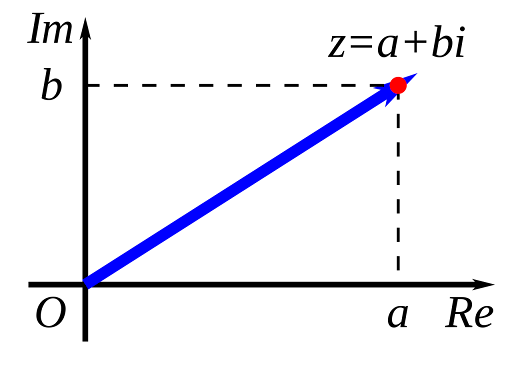
\includegraphics[width=\textwidth,keepaspectratio]{rectangular_form.png}
                \end{minipage}\hfill
                \begin{minipage}{0.40\textwidth}
                    Rectangular form
                    \label{fig:rectangular_form.png}
                \end{minipage}
            \vspace{-0.5cm}
            \begin{minipage}{0.58\textwidth}
                \centering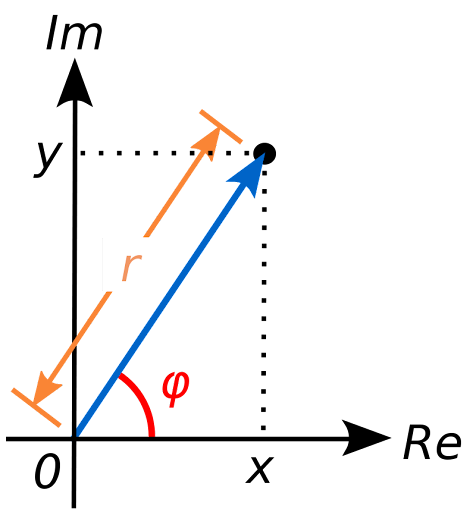
\includegraphics[height=4cm,width=\textwidth,keepaspectratio]{polar_form.png}
            \end{minipage}\hfill
            \begin{minipage}{0.40\textwidth}
                Polar form
                \label{fig:polar_form.png}
            \end{minipage}
        \end{column}
    \end{columns}
\end{frame}

\begin{frame}[t]{Reference material}
    \framesubtitle{}
    \Large
    \begin{itemize}
        \item \href{https://www.youtube.com/watch?v=Y_Ac6KiQ1t0&list=PL49CF3715CB9EF31D&index=17}{Lecture 17}
        \item \textit{"Linear Algebra and Applications", pdf pages 205--221 }\\ Orthogonal Bases and Gram-Schmidt
        \item \href{https://www.youtube.com/watch?v=eib8uAlzegc&list=PLkZjai-2Jcxlg-Z1roB0pUwFU-P58tvOx&index=20}{Gram-Schmidt Process | Lectures 19 and 20}\\ Video from Matrix Algebra for Engineers course
        \item \href{https://www.youtube.com/watch?v=J41Ypt6Mftc}{QR Factorization}
    \end{itemize}
\end{frame}

\fbckg{fibeamer/figs/last_page.png}
\frame[plain]{}

\end{document}